\section{Entwurf}
\subsection{Zielplattform}
Die Anwendung soll auf Windows PC lauffähig sein.\\
Windows 10 wird als Standard System vorausgesetzt.\\
Als Programmiersprache wird Java 8 verwendet und mit der IDE Eclipse wird der Quellcode geschrieben.\\
Als Datenbank wird eine lokale SQLite Datenbank eingesetzt.\\

% ===============================================
\subsection{Architekturdesign}
Ich teile die Entwicklung des Programms in 3 Ebenen.\\
\begin{itemize}
\item{Datenbank}
\item{Logik}
\item{Oberfläche}
\end{itemize}
Die Einteilung dient der Übersicht in der Erstellung des Quellcodes und für eine bessere Dynamik.\\
So kann z.B. durch die Abgrenzung der Datenbankebene von der Logikebene schnell ein anderes Datenbanksystem als Grundlage gewechselt werden. \\
Zum Beispiel von \textbf{SQLite} zu \textbf{MySql Server}.\\
Die Trennung von Logik zu Oberfläche bietet den Vorteil, dass spätere Anpassungen in der Bedienung oder ein komplett neues Design zügig geändert werden kann ohne die Logik umschreiben zu müssen. Außerdem könnten die Ebenen auch separat in anderen Projekten wiederverwendet werden.\\



\subsection{Entwurf der Benutzeroberflächen}
Ein GUI ist geeignet, um schnell und bedienerfreundlich die Anforderungen an das Programm zu erfüllen.\\
Zum Erstellen der Benutzeroberfläche verwende ich den Window Builder, der als Addon in der Eclipse IDE kostenlos dazu geladen werden kann.\\
Die Informationen über die einzelnen Bücher werden, in einem Grid gelistet, dargestellt.\\
\begin{figure}[h]
\begin{center}
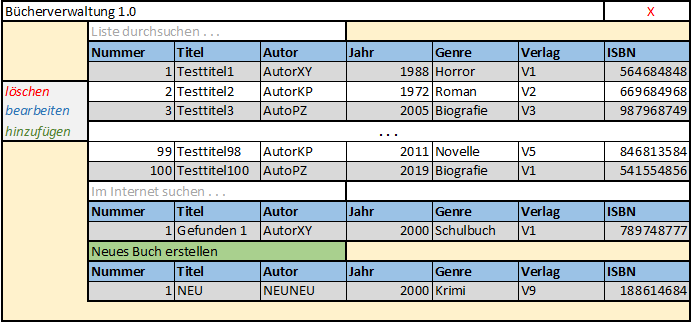
\includegraphics[width=15cm]{img/entwurf.png}
\caption{Entwurf der Benutzeroberfläche}
\label{entwurf_gui}
\end{center}
\end{figure}


\subsection{Datenmodell}
Zu Beginn des Programms wird eine Verbindung zur Datenbank hergestellt.\\
Danach werden Listen erzeugt und diese mit den Daten aus der Datenbank gefüllt.\\
Während der Laufzeit werden alle Darstellungen und interne Suchen über die Listen vollzogen.\\
Änderungen, wie das bearbeiten einzelner Felder, das Löschen oder das Hinzufügen werden nach aktualisieren der Listen in die Datenbank geschrieben.\\
Zum Programm Ende wird die Verbindung zur Datenbank getrennt.\\
In der folgenden Abbildung wird ein Modell des Programms dargestellt.\\

\begin{figure}[h]
\begin{center}
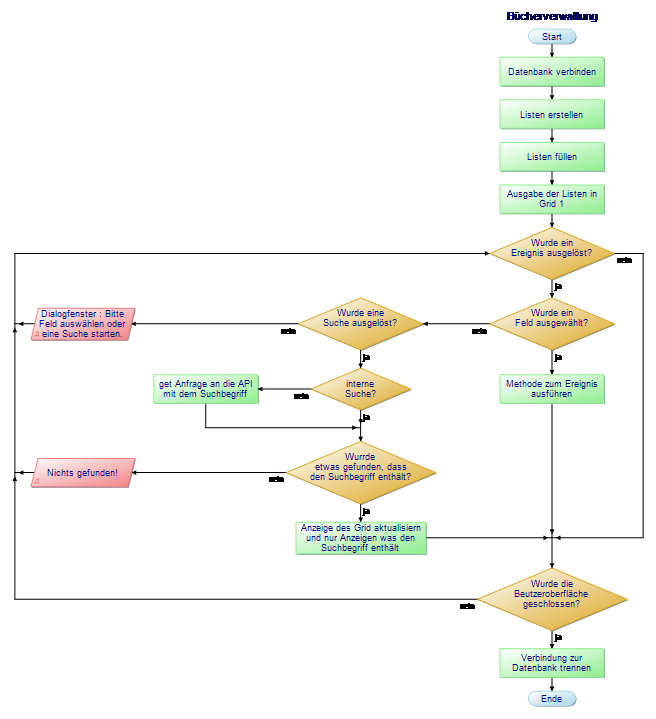
\includegraphics[width=17cm]{img/mainpap.png}
\caption{Programmablaufplan}
\label{entwurf_pap}
\end{center}
\end{figure}




